% 学習結果説明（材料別の温度シフト GPR：厚みごとの比較。05 フォルダのデータ。用語集と図の見方）
% 05_材料ごとの機械学習データと予測検証データ フォルダで「lualatex 学習結果説明_厚みごとの温度シフト.tex」を2回実行すると PDF を作り直せる（TeX Live の LuaLaTeX を使用）。
% 図は、各材料フォルダの <材料フォルダ>_学習結果/条件平均の入力/厚みごとの比較/ の PNG を相対パスで読み込む。
\documentclass[paper=a4paper,fontsize=10.5pt,line_length=44zw,number_of_lines=38]{jlreq}
\usepackage[haranoaji]{luatexja-preset}
\usepackage{amsmath}
\usepackage{graphicx}
\usepackage{booktabs}
\usepackage{tabularx}
\usepackage{enumitem}
\usepackage{float}
\usepackage{xcolor}
\usepackage[hidelinks,bookmarksnumbered]{hyperref}

\newcommand{\file}[1]{\texttt{\detokenize{#1}}}
\newcommand{\gd}{\dot{\gamma}}
\newcommand{\Tff}{T_{\mathrm{ff}}}
\newcommand{\Tset}{T_{\mathrm{set}}}
\newcommand{\Eh}{E_{h}}
\newcommand{\Ev}{E_{v}}
\newcommand{\PIII}{P3\_3}
\newenvironment{termlist}{\begin{itemize}[label=・,leftmargin=1\zw,labelwidth=1\zw,labelsep=0pt,itemsep=0.4ex,topsep=0.6ex,parsep=0pt]}{\end{itemize}}
\newcommand{\term}[1]{\item \textbf{#1}：}
\newenvironment{points}{\begin{itemize}[label=$\triangleright$,leftmargin=1.5\zw,itemsep=0.3ex,topsep=0.5ex,parsep=0pt]}{\end{itemize}}
\newcommand{\pt}[1]{\item \textbf{#1}：}
\renewcommand{\arraystretch}{1.25}

\title{厚みごとに見た温度シフトの説明\\[0.6ex]{\large 材料別の温度シフト GPR（05 のデータ）：厚みごとの確認、シフトに使う温度、厚みごとに学習するか総合データで学習するか（機械学習・統計を初めて学ぶ人向け）}}
\author{}
\date{2026年10月22日}

\begin{document}
\maketitle
{\small\tableofcontents}

% =====================================================================
\section{この文書について}

この文書は、材料別の温度シフト GPR（説明書 \file{学習結果説明_材料別温度シフトGPR.pdf}）の学習結果を、\textbf{キャビティ厚みごと}に調べ直した結果を、機械学習や統計を初めて学ぶ人でも読めるように説明したものです。調べたのは、次の 3 つの問いです（ユーザーの依頼）。

\begin{enumerate}[itemsep=0.3ex,topsep=0.5ex]
\item 厚みごとの「せん断速度 ― 粘度」の学習結果で、\textbf{温度シフトファクターが効いているか}。
\item 厚みごとに見たとき、シフトに使う温度は、\textbf{流動中樹脂温度 $\Tff$ と加熱シリンダ温度 $\Tset$ のどちらが適しているか}。
\item 学習用 5data・検証用 3data はそのままで、\textbf{厚みごとに学習するのと、全厚みを含めた総合データで学習するのと、どちらがよいか}。
\end{enumerate}

\begin{points}
\pt{対象の結果}材料ごとに \file{<材料フォルダ>_学習結果/条件平均の入力/厚みごとの比較/}（例：\file{01_バージンPP再々実験/01_バージンPP再々実験_学習結果/条件平均の入力/厚みごとの比較/}）。図 57 枚、CSV 33 個（3 材料の合計）。図は、同じフォルダの \file{highres/} にも 600 dpi で保存されます。4章の図のファイル名は、このフォルダの中の名前です。
\pt{読み方}2章で何をしたかをつかみ、分からない言葉は3章の用語集で調べてください。4章で図の見方、5章で表の見方、6章で結論を説明します。\textbf{結論だけを知りたいときは、6章から読んでください}。
\pt{ノート}\file{01_機械学習コードフォルダ} の \file{材料別_温度シフトGPR_ARD対応Matern52＋線形＋ホワイトノイズ_厚みごとの比較.ipynb} です（元のノートとは別のノート）。元のノートで学習済みのモデル（\file{学習済みモデル_<モデル>.joblib}）と予測値の CSV を読むので、\textbf{先に元のノートを実行しておく必要があります}。実行は約 10〜13 分です（大部分は、厚みごとのプロファイル尤度と、厚みごとのモデルの学習）。
\pt{実行のしかた}ノートを \file{_tmp/} にコピーし（設定を変えるなら、そのコピーの設定エリアで）、リポジトリ直下で \file{uv run python 04_補助スクリプト/run_nb.py _tmp/<コピー>.ipynb} を実行します。元のノートと同じく、成果物のノートは実行結果ごと上書きしません。
\pt{発表資料}同じ結果を、発表資料 \file{学習結果報告書作成_261015/パワーポイント/報告書B_5章以降_発表資料.pptx} の 6 章（厚みごとの確認、シフトに使う温度）・7 章（厚みごとに学習したモデルとの比較）・最後の 1 枚（結論）にまとめました。発表資料では、流動中樹脂温度 $\Tff$ を「金型内樹脂最高温度 $T$」と呼んでいます（同じもの）。
\pt{記号表}記号・モデル名・列名の一覧は、\file{results/学習結果説明_記号表.pdf} の「材料別 GPR」の章にあります。
\pt{作り直し方}\file{05_材料ごとの機械学習データと予測検証データ} フォルダで \texttt{lualatex 学習結果説明\_厚みごとの温度シフト.tex} を2回実行すると、この PDF を作り直せます（数値を CSV から入れ直すときは \file{uv run python 04_補助スクリプト/build_report_mat_thick.py}）。
\pt{ノートの判定}ノートの各節の最後に、\file{>> 判定：OK}（想定どおり）か \file{>> 判定：★要確認}（想定と違う、または注意が要る点）が出ます。今回は、OK が 95 個、★ が 7 個でした（一覧は \file{判定の一覧.csv}）。6章に、★ の意味を書きました。
\end{points}

% =====================================================================
\section{何をしたか（概要）}

\subsection{2 つのシフトのモデル}
元のノートで学習した、次の 3 つのモデル（条件平均の入力）を使います。どちらのシフトのモデルも\textbf{両方の温度を使っています}。違うのは、\textbf{シフトに使う温度}だけです。
\begin{table}[H]
\caption{比べたモデル。$f$ はガウス過程、$a_h$・$a_v$ は横・縦のシフトファクター}\label{tab:model}
\small
\begin{tabularx}{\linewidth}{@{}l>{\raggedright\arraybackslash}X@{}}
\toprule
モデル & 式と考え方 \\
\midrule
B\_Tset & $\ln\eta=\ln a_v(\Tset)+f(\ln\gd+\ln a_h(\Tset),\ \ln\PIII,\ \ln\Tff)$。加熱シリンダ温度でシフトし、流動中樹脂温度は GP の入力に入れる \\
B\_Tff & $\ln\eta=\ln a_v(\Tff)+f(\ln\gd+\ln a_h(\Tff),\ \ln\PIII,\ \Tset)$。流動中樹脂温度でシフトし、加熱シリンダ温度は GP の入力に入れる。発表資料で使ったモデル \\
C（基準） & $\ln\eta=f(\ln\gd,\ \ln\PIII,\ \ln\Tff,\ \Tset)$。シフトなし \\
\bottomrule
\end{tabularx}
\end{table}
全厚みの 5data で学習した係数（\textbf{全厚み共通の係数}）は次のとおりです：PP は B\_Tset が $\Eh$ 9・$\Ev$ 14 kJ/mol、B\_Tff が $\Eh$ 8・$\Ev$ 20 kJ/mol、粉砕材混合 PP は B\_Tset が $\Eh$ 3・$\Ev$ 0 kJ/mol、B\_Tff が $\Eh$ 6・$\Ev$ 17 kJ/mol、GPPS は B\_Tset が $A_{1,h}$ 3・$A_{1,v}$ 6、B\_Tff が $A_{1,h}$ 3・$A_{1,v}$ 8。

\subsection{3 つの問いの調べ方}
\begin{table}[H]
\caption{調べ方の一覧（ノートの節の番号）}\label{tab:method}
\small
\begin{tabularx}{\linewidth}{@{}l>{\raggedright\arraybackslash}X@{}}
\toprule
問い & 調べ方 \\
\midrule
1 シフトが効いているか（4 節） & 全厚み共通の係数のまま、厚みごとに、①温度の順序（同じ $\gd$ で低温ほど高粘度か）、②温度による粘度の比 $R$ の実測と予測、③換算前後の重ね合わせのずれ、の 3 つを見る。3 つとも満たせば ○、予測の順序が逆なら ×、それ以外は △ \\
2 シフトに使う温度（5〜8 節） & (a) \textbf{重ね合わせ}：厚みごとに係数を決め直したときの、最小のずれ（データだけで決まる）。(b) \textbf{対数周辺尤度}：厚みごとの 5data だけで B\_Tset・B\_Tff を学習し、最大の LML の差 $\Delta L$ を比べる。(c) \textbf{検証データの予測誤差}：元のノートの 3data の予測を、厚みごとに集計する。3 つの多数決で、厚みごとに「$\Tff$／$\Tset$／差なし」を決める \\
3 厚みごとか総合か（9 節） & 厚みごとの 5data だけで B\_Tset・B\_Tff・C を学習し直し（係数は (b) で決めたもの）、同じ厚みの 3data を予測する。総合データ（全厚みの 5data）で学習した元のモデルの予測と、同じ 3data で比べる \\
\bottomrule
\end{tabularx}
\end{table}

\subsection{判定の基準}
\begin{points}
\pt{比の大きさが一致}$|\ln R_{\text{予測}}-\ln R_{\text{実測}}|$ が、モデルのノイズの標準偏差（約 0.04〜0.05。粘度で約 4〜5\%）以内。
\pt{(a) の差}ずれの差が 0.5 ポイント以上なら、小さいほうの温度が適している（それ未満は差なし）。
\pt{(b) の差}$|\Delta L|\ge$ 3.0 なら、LML の大きいほうの温度が適している（尤度比検定の 5\% 基準と同じ目安）。
\pt{(c) の差}予測誤差の差が 1.0 ポイント以上なら、小さいほうが適している。
\pt{厚みごとか総合か}予測誤差が、どちらかの方式で、多くの厚みで 1 ポイント以上小さければ、その方式を勧める。差が小さければ、データの量と使いやすさから総合データを勧める。
\end{points}
基準の値は、ノートの設定エリア（\file{A_CLEAR}・\file{DL_CLEAR}・\file{ERR_CLEAR}）で変えられます。

% =====================================================================
\section{用語集}
\begin{termlist}
\term{キャビティ厚み $H$}金型の流路（平板）の厚み。PP・粉砕材混合 PP は 0.5・1.0・1.5・2.0 mm、GPPS は 1.0・1.5・2.0 mm。モデルの入力には入れていない（厚みの違いは \PIII\ を通して入る）。
\term{温度シフトファクター}温度による粘度曲線のずれ。横（$a_h$、せん断速度の向き）と縦（$a_v$、粘度の向き）がある。
\term{全厚み共通の係数・厚みごとの係数}全厚みのデータで 1 組だけ決めた係数（元のモデル）と、厚みごとに決め直した係数。
\term{温度による粘度の比 $R$}同じせん断速度で、最低温度の粘度を最高温度の粘度で割った値。1 より大きければ低温ほど高粘度。温度の違う点のせん断速度はそろっていないので、成形条件ごとの平均を、$\ln\gd$ の重なる範囲の共通の格子（50 点）で内挿し、$R=\exp(\text{平均}[\ln\eta_{\text{low}}-\ln\eta_{\text{high}}])$ とする。予測の $R$ は、各条件でのモデルの予測平均から、同じ手順で出す。
\term{重ね合わせのずれ}温度ごとの点を係数で換算したとき、1 本の曲線にどれだけ重なるか。厚みごとに、換算した $\ln\gd$ に対する 3 次式を当てはめ、その残差の標準偏差を、粘度の \% に直した値（$(e^{s}-1)\times100$）。小さいほどよく重なる。
\term{換算前・換算後}換算前は、係数 0（シフトなし）。換算後は、係数でずらした後。
\term{対数周辺尤度（LML）・$\Delta L$}モデルがデータにどれだけ合うかを表す数（大きいほど合う）。$\Delta L=\mathrm{LML}(\text{B\_Tff})-\mathrm{LML}(\text{B\_Tset})$。同じデータで学習した 2 つのモデルの比較なので、差が大きければ、そのデータでは一方がよく合う。
\term{係数 0 との差}シフトの係数を入れたモデルと、係数 0 のモデルの LML の差。3.0 以上なら、シフトを入れた効果が認められる目安。
\term{プロファイル尤度・取り直し}係数を格子で振り、各点で GP を学習して LML を求め、最大の点を採る方法。最良の点の近くを細かい格子で計算し直し、最良の点が動いたら、もう一度取り直す（\file{MAX_REFINE} 回まで）。取り直しが収束しないのは、尤度の面が平らで、係数が決まりにくいとき。
\term{多数決}(a)(b)(c) の 3 つの判定のうち、2 つ以上が同じ温度なら、その温度。そうでなければ「差なし」。
\term{厚みごとのモデル・総合データのモデル}1 つの厚みの 5data だけで学習したモデルと、全厚みの 5data で学習したモデル（元のノートのモデル）。
\term{低速側・高速側・外挿}3data の射出速度 3・5 mm/s（厚い板だけ）と 280・320 mm/s。どちらも、5data の範囲（10〜240 mm/s）の外への予測（外挿）。
\term{予測誤差（\%）}3data の $\ln\eta$ の RMSE を、粘度の \% に直した値（$(e^{\mathrm{RMSE}}-1)\times100$）。
\term{95\% 予測区間に入った割合}3data の点が、予測の 95\% 区間に入った割合。0.95 に近いほど、ばらつきの見積もりが正しい。
\end{termlist}

% =====================================================================
\section{図の見方}

図は材料ごとのフォルダにあります。ここでは主に PP の図で見方を説明し、ほかの材料の結果は文中と5章の表で示します。

\subsection{図1：厚みごとの学習結果（PP・厚み 2.0 mm）}
\begin{figure}[H]
\centering
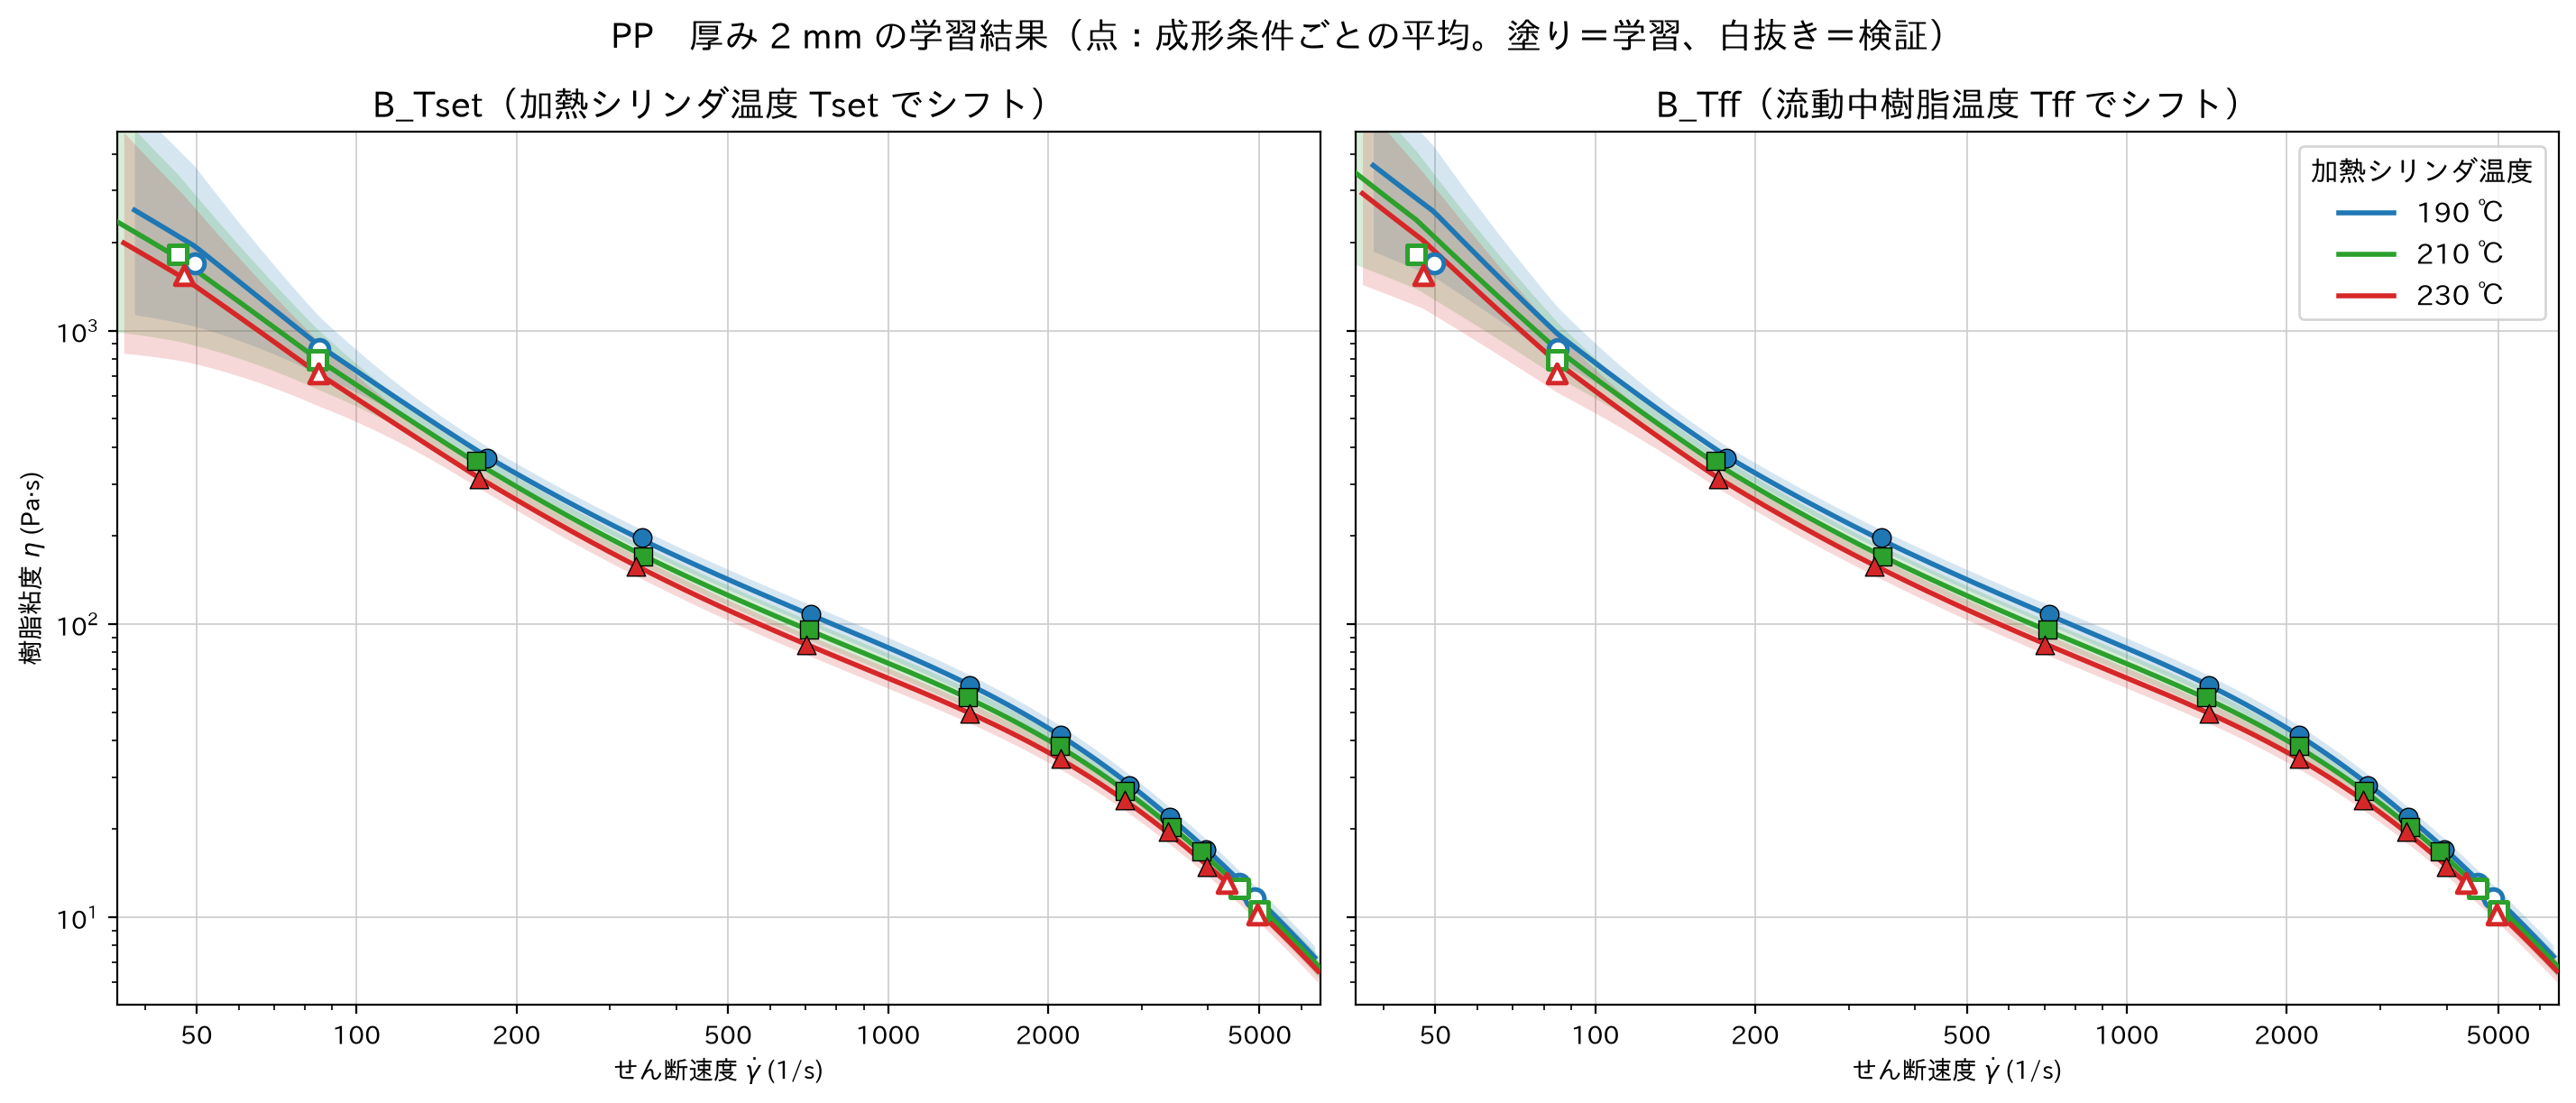
\includegraphics[width=0.95\linewidth]{01_バージンPP再々実験/01_バージンPP再々実験_学習結果/条件平均の入力/厚みごとの比較/学習結果_厚み2mm.png}
\caption{左が B\_Tset、右が B\_Tff。点は成形条件ごとの平均（塗り＝学習、白抜き＝検証）、線は加熱シリンダ温度ごとの予測平均、帯は 95\% 予測区間}
\end{figure}
\begin{points}
\pt{何を示す図か}全厚み共通の係数で学習したモデルの予測を、1 つの厚みだけ取り出して描いた図です（ファイル：\file{学習結果_厚み<厚み>mm.png}。厚みごとに 1 枚）。
\pt{軸と記号}両対数。横軸がせん断速度 $\gd$、縦軸が粘度 $\eta$。色と形が加熱シリンダ温度（青 190 ℃・緑 210 ℃・赤 230 ℃。GPPS は 200・220・240 ℃）。曲線の入力（\PIII・$\Tff$）は、同じ厚み・温度の成形条件の値を、せん断速度で内挿したもの。
\pt{見るポイント}3 本の線が、実測の点と同じ順序（低温が上）・同じ間隔で並ぶか。白抜きの点（学習していない低速側・高速側）が帯の中にあるか。
\pt{今回の結果}PP の 2.0 mm では、どちらのモデルも 3 本の線が実測と同じ順序で並び、間隔も合います（温度による粘度の比 $R$：実測 1.22、B\_Tff の予測 1.24）。低速側（左端の白抜き）は外挿なので、帯が広がります。
\end{points}

\subsection{図2：温度による粘度の比 $R$（PP）}
\begin{figure}[H]
\centering
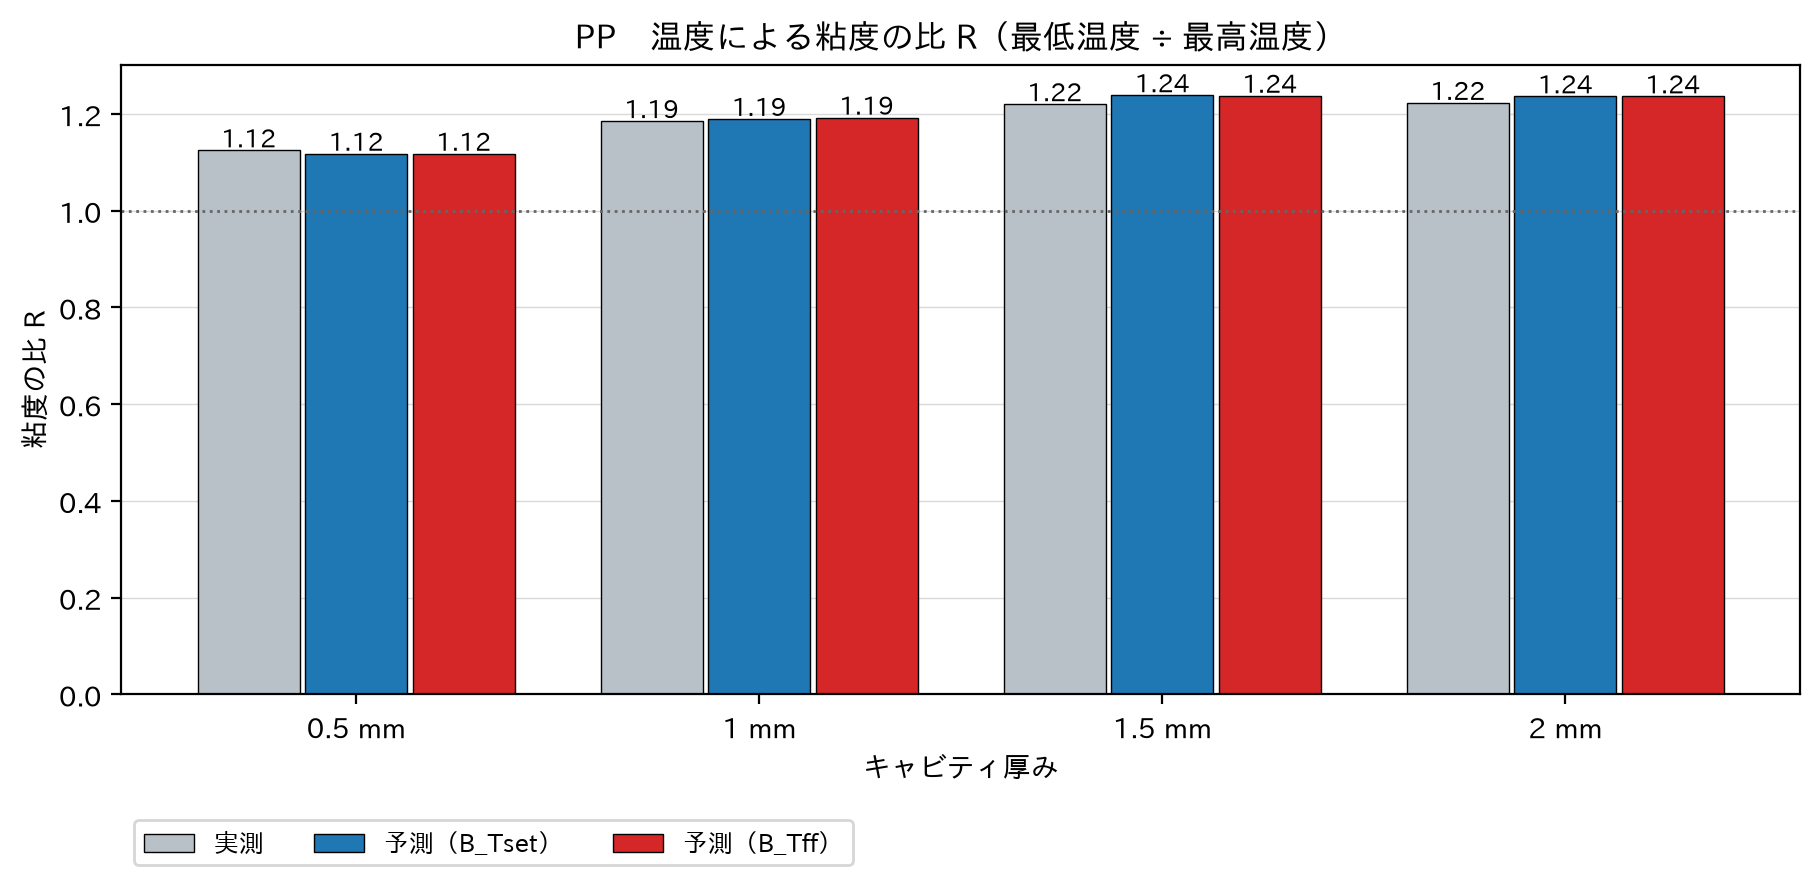
\includegraphics[width=0.95\linewidth]{01_バージンPP再々実験/01_バージンPP再々実験_学習結果/条件平均の入力/厚みごとの比較/温度による粘度の比.png}
\caption{厚みごとの $R$（灰：実測、青：B\_Tset の予測、赤：B\_Tff の予測）}
\end{figure}
\begin{points}
\pt{何を示す図か}同じせん断速度で、最低温度の粘度が最高温度の何倍かを、厚みごとに実測と予測で比べた図です（ファイル：\file{温度による粘度の比.png}）。
\pt{軸と記号}縦軸が $R$（1 より大きければ低温ほど高粘度。点線が 1）。横軸がキャビティ厚み。
\pt{見るポイント}予測の棒が、実測の棒と同じ高さか。
\pt{今回の結果}3 材料・全厚みで、予測の $R$ は実測とよく合いました（$|\ln R_{\text{予測}}-\ln R_{\text{実測}}|$ は最大 0.034。ノイズの標準偏差 約 0.04 より小さい）。PP では、$R$ は厚いほど大きく（1.12〜1.22）、モデルもこの傾向を表しています。B\_Tset と B\_Tff の差は、この図ではほとんどありません。
\end{points}

\subsection{図3：重ね合わせ（PP・厚み 0.5 mm・全厚み共通の係数）}
\begin{figure}[H]
\centering
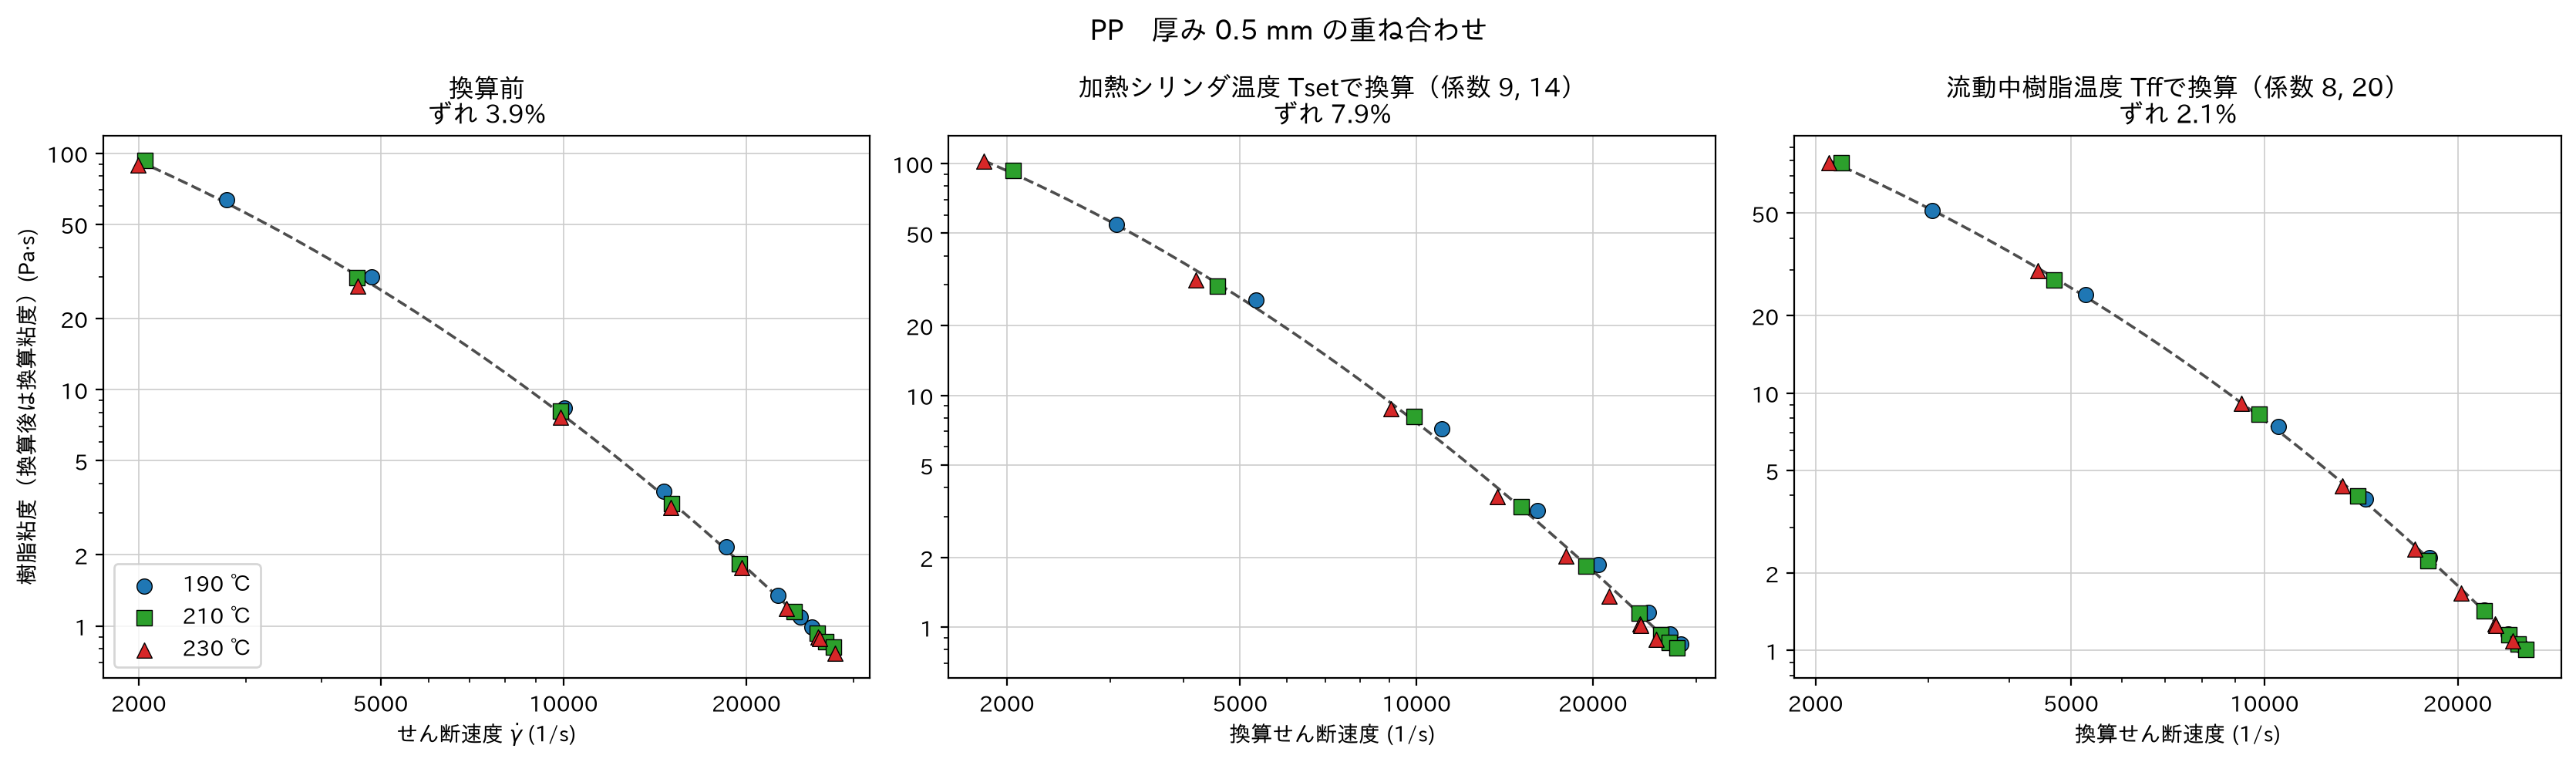
\includegraphics[width=0.95\linewidth]{01_バージンPP再々実験/01_バージンPP再々実験_学習結果/条件平均の入力/厚みごとの比較/重ね合わせ_学習済みの係数_厚み0.5mm.png}
\caption{左から、換算前、加熱シリンダ温度で換算、流動中樹脂温度で換算。破線は 3 次式}
\end{figure}
\begin{points}
\pt{何を示す図か}全厚み共通の係数で、温度ごとの点を換算（シフト）したとき、1 本の曲線に重なるかを見る図です（ファイル：\file{重ね合わせ_学習済みの係数_厚み<厚み>mm.png}。厚みごとに決め直した係数の図は \file{重ね合わせ_厚みごとの係数_厚み<厚み>mm.png}）。
\pt{軸と記号}両対数。横軸が（換算）せん断速度、縦軸が（換算）粘度。色と形が加熱シリンダ温度。図の上の「ずれ」が、3 次式からのずれ（粘度の \%）。
\pt{見るポイント}換算後に、温度の違う点が破線の近くに集まるか。ずれが換算前より小さいか。
\pt{今回の結果}0.5 mm は温度の効果が小さい厚みです（換算前のずれ 3.9\%）。流動中樹脂温度で換算すると 2.1\% に減りますが、加熱シリンダ温度で換算すると 7.9\% に\textbf{増えます}。加熱シリンダ温度の全厚み共通の係数は、温度の効果が大きい厚肉に合わせて決まっていて、薄肉では換算しすぎる（230 ℃ の点が左にずれすぎる）ためです。
\end{points}

\subsection{図4：重ね合わせのずれ（PP・全厚み共通の係数）}
\begin{figure}[H]
\centering
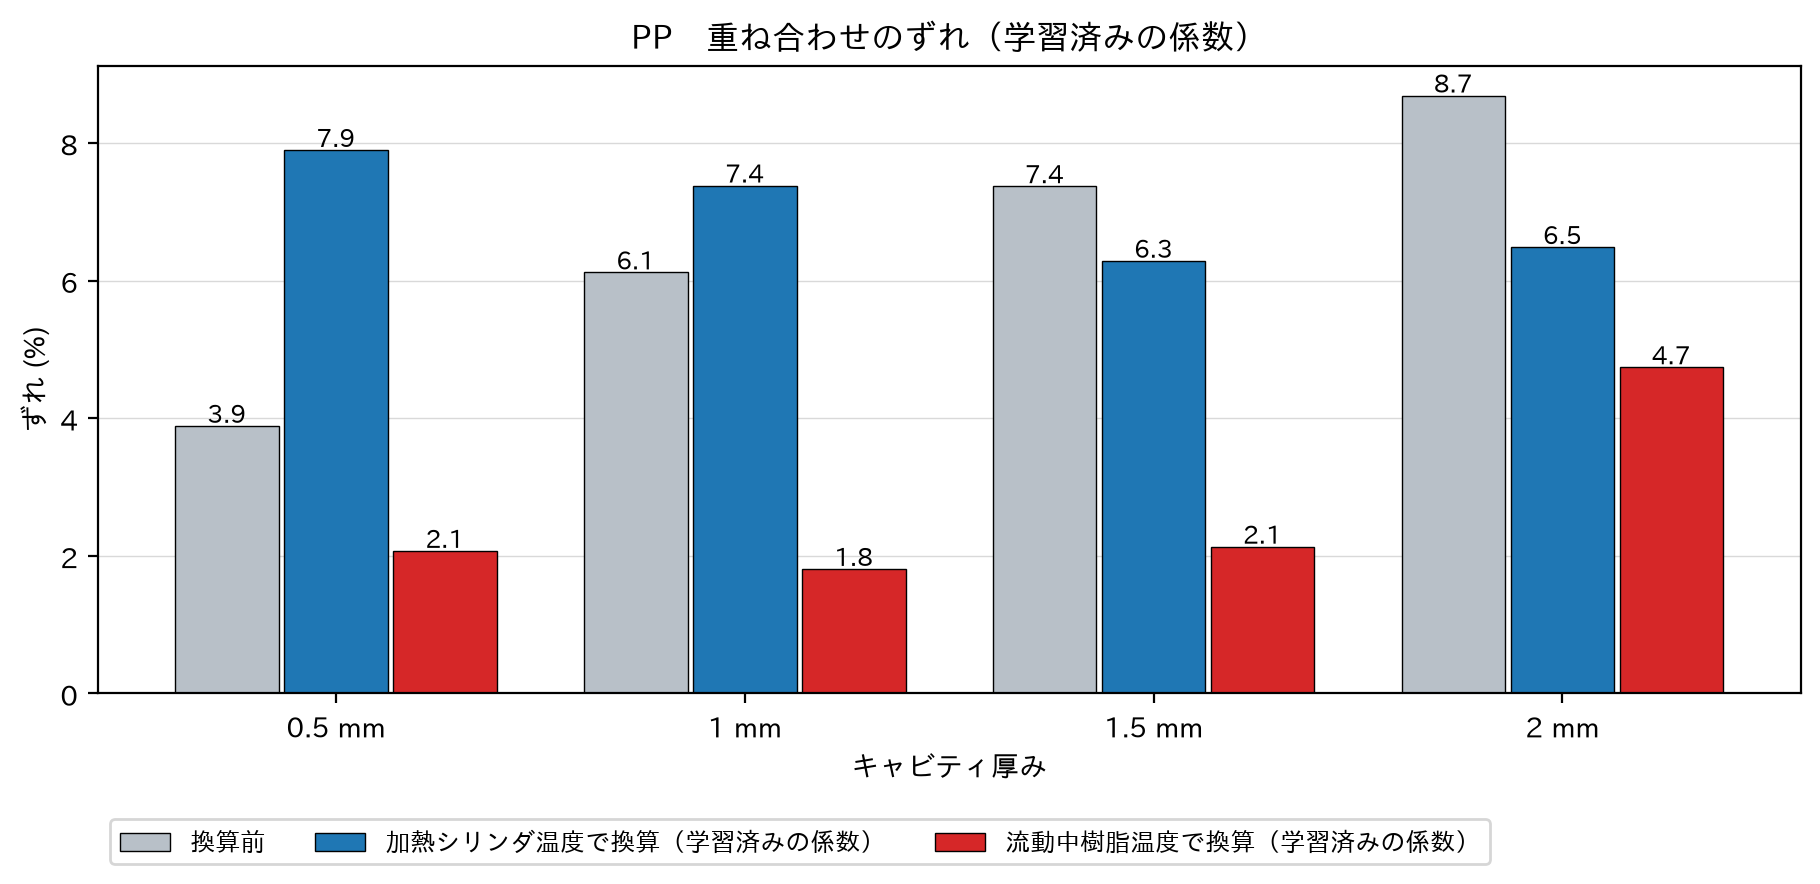
\includegraphics[width=0.95\linewidth]{01_バージンPP再々実験/01_バージンPP再々実験_学習結果/条件平均の入力/厚みごとの比較/重ね合わせのずれ_学習済みの係数.png}
\caption{厚みごとの、換算前（灰）・加熱シリンダ温度で換算（青）・流動中樹脂温度で換算（赤）のずれ}
\end{figure}
\begin{points}
\pt{何を示す図か}図3 のずれを、全厚みについて並べた図です（ファイル：\file{重ね合わせのずれ_学習済みの係数.png}）。
\pt{軸と記号}縦軸がずれ（粘度の \%）。横軸がキャビティ厚み。
\pt{見るポイント}赤・青の棒が、灰の棒より低いか（換算でずれが減るか）。
\pt{今回の結果}流動中樹脂温度で換算すると、3 材料の 11 厚みすべてで、ずれが減りました。加熱シリンダ温度では、PP の 0.5・1.0 mm、粉砕材混合 PP の全厚みで増えました（5 章の表 4）。このため、全厚み共通の係数での判定（問い 1）は、B\_Tff が全厚みで ○、B\_Tset はこれらの厚みで △ です。なお、B\_Tset でも、予測の $R$ は実測と合っています（図2）。B\_Tset では、温度の効果の多くを、GP の入力の $\Tff$ が担っているためです。
\end{points}

\subsection{図5：(a) 厚みごとに係数を決め直したときの重ね合わせのずれ（PP）}
\begin{figure}[H]
\centering
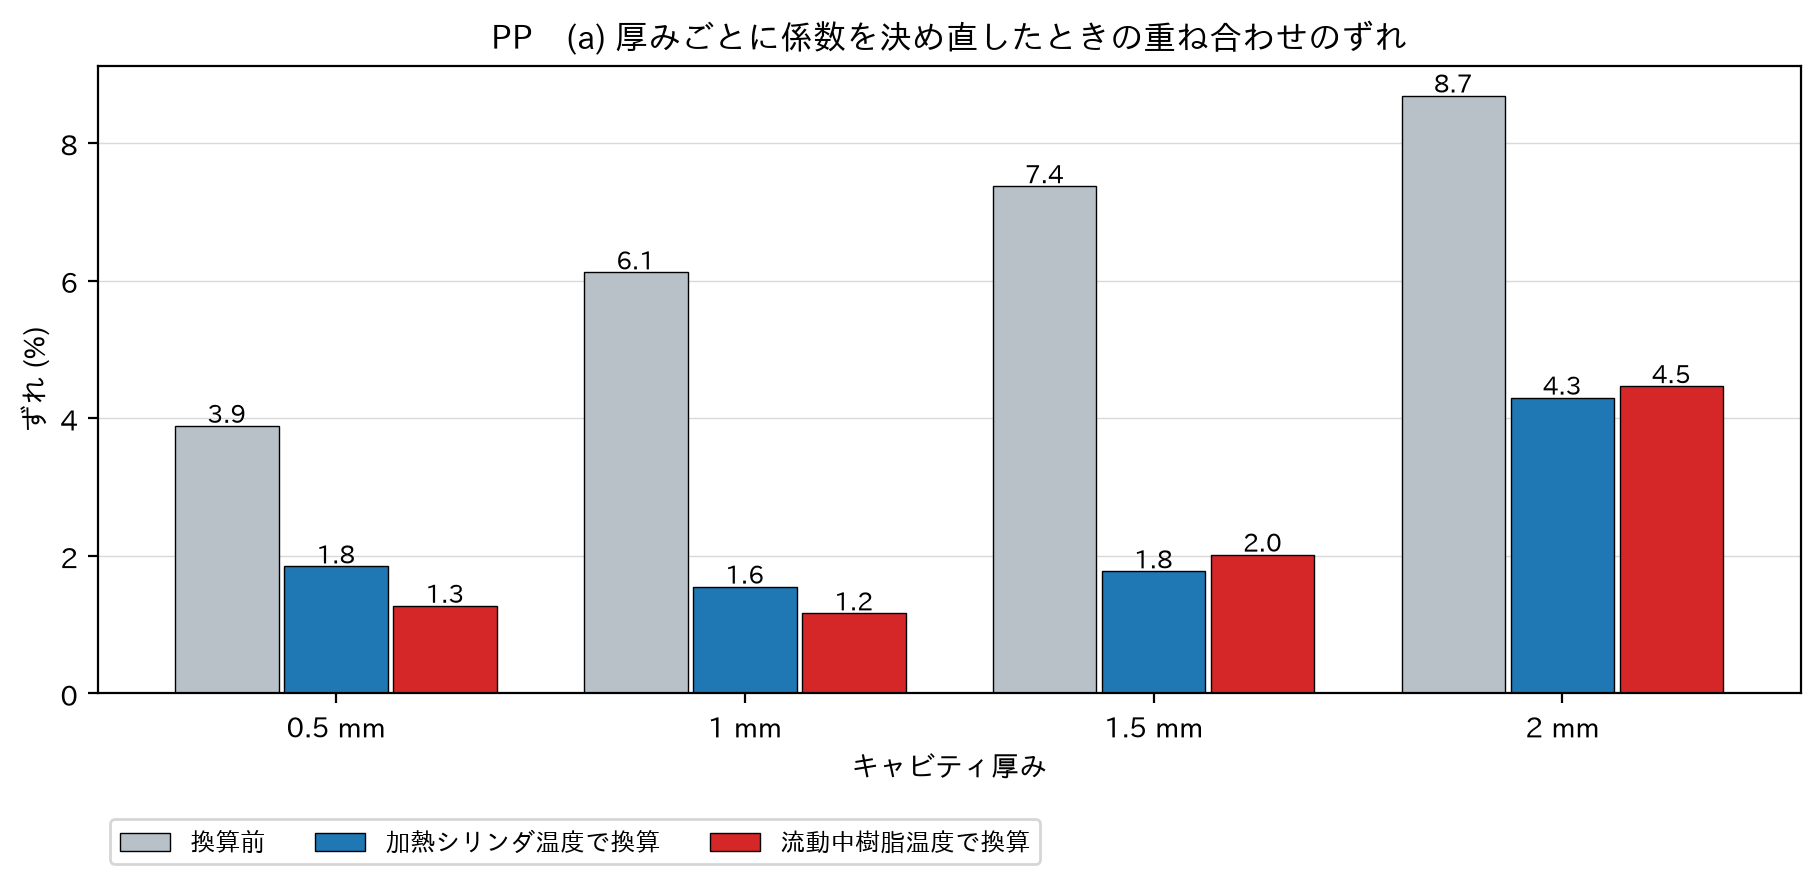
\includegraphics[width=0.95\linewidth]{01_バージンPP再々実験/01_バージンPP再々実験_学習結果/条件平均の入力/厚みごとの比較/重ね合わせのずれ_厚みごとの係数.png}
\caption{厚みごとに、ずれが最小になる係数を探したときのずれ}
\end{figure}
\begin{points}
\pt{何を示す図か}厚みごとに係数（横・縦）を決め直し、どちらの温度で換算したほうがよく重なるかを比べる図です（基準 (a)。ファイル：\file{重ね合わせのずれ_厚みごとの係数.png}）。データの点だけで決まり、GP のモデルを使いません。
\pt{軸と記号}図4 と同じ。
\pt{見るポイント}青と赤の棒の差が 0.5 ポイント以上あるか（あれば、低いほうの温度が適する）。
\pt{今回の結果}係数を決め直すと、どちらの温度でも、ずれは換算前の 1/2〜1/4 に減ります。差が 0.5 ポイント以上あったのは、各材料で最も薄い厚み（PP・粉砕材混合 PP の 0.5 mm、GPPS の 1.0 mm）だけで、いずれも流動中樹脂温度が小さい結果でした。ほかの厚みは差なしです。
\end{points}

\subsection{図6：(b) 厚みごとの対数周辺尤度の差（PP）}
\begin{figure}[H]
\centering
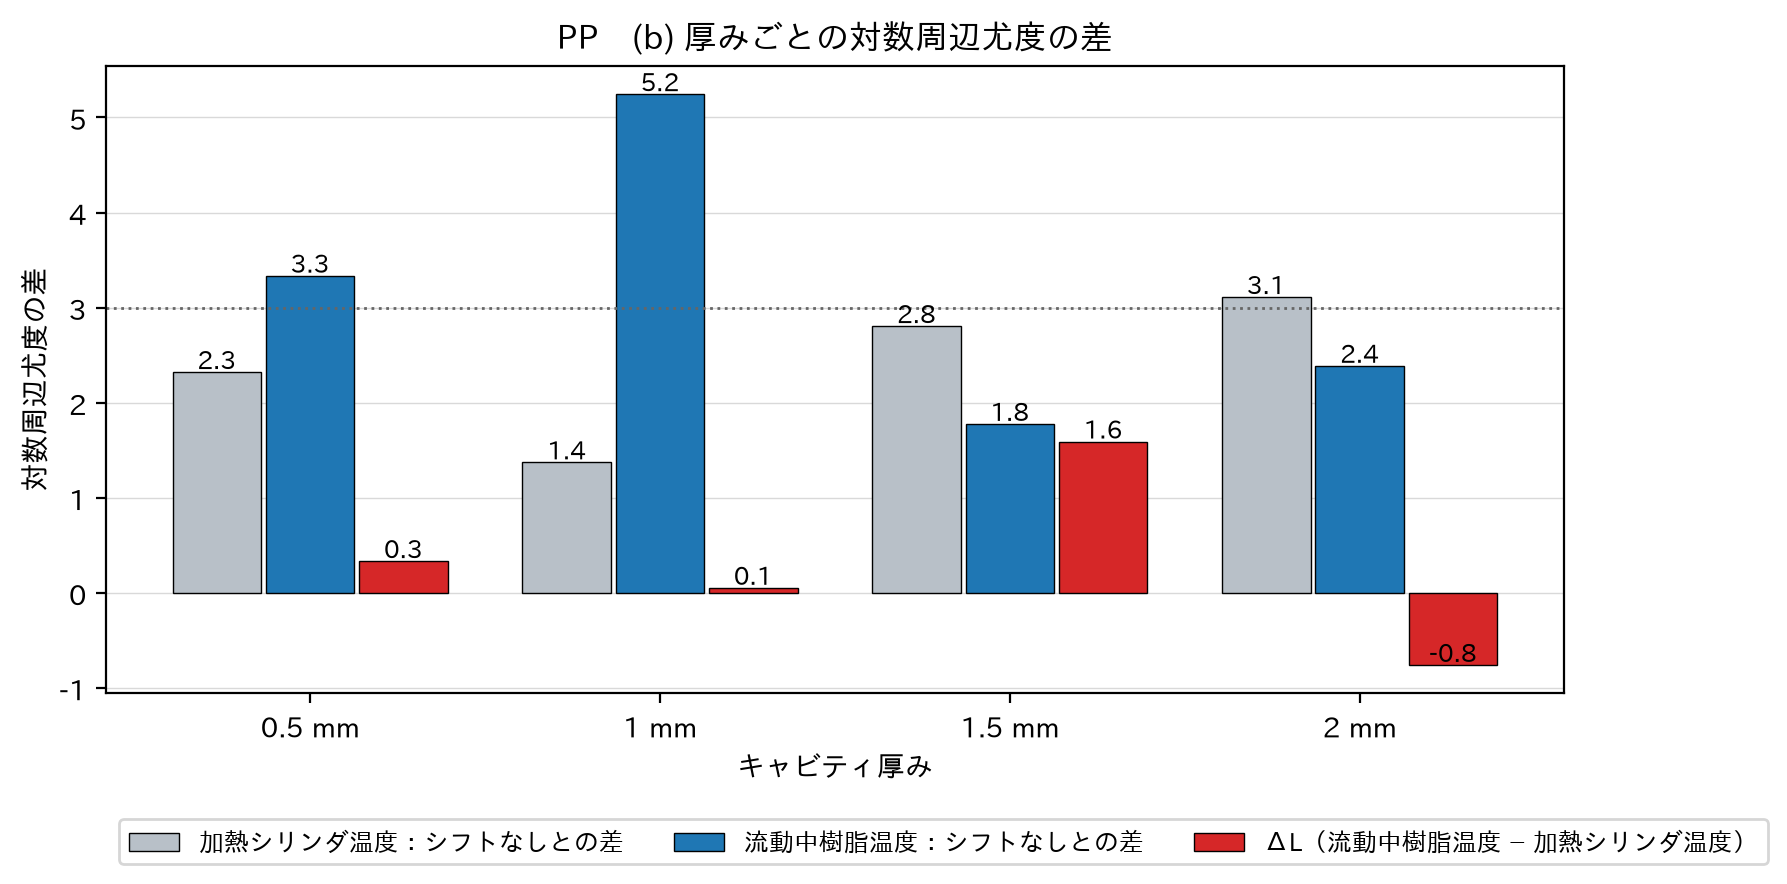
\includegraphics[width=0.9\linewidth]{01_バージンPP再々実験/01_バージンPP再々実験_学習結果/条件平均の入力/厚みごとの比較/対数周辺尤度の差_厚みごと.png}
\caption{灰：B\_Tset の係数 0 との差、青：B\_Tff の係数 0 との差、赤：$\Delta L$（B\_Tff − B\_Tset）}
\end{figure}
\begin{points}
\pt{何を示す図か}厚みごとの 5data だけで、2 つのモデルの係数をプロファイル尤度で決め、データへの合い具合（LML）を比べた図です（基準 (b)。ファイル：\file{対数周辺尤度の差_厚みごと.png}）。
\pt{軸と記号}縦軸が LML の差。点線が 3.0（効果が認められる目安）。
\pt{見るポイント}赤の棒が $+3$ を超えるか（$\Tff$ が適する）、$-3$ を下回るか（$\Tset$ が適する）。灰・青の棒が 3 を超えるか（その厚みだけで、シフトの効果が認められるか）。
\pt{今回の結果}3 材料・全厚みで $|\Delta L|$ は最大 1.6 で、基準の 3 に届きません（すべて差なし）。係数 0 との差も 0.9〜5.2 と小さく、3 以上は 22 組中 7 組だけです。厚みごとの学習データは成形条件 21〜24 しかなく、1 つの厚みだけでは、シフトの係数がよく決まりません。決まった係数も厚みで大きく変わります（例：PP の 2.0 mm の B\_Tset は $\Ev$ が -36 kJ/mol で、細かい格子の取り直しが収束しませんでした。ノートの ★）。
\end{points}

\subsection{図7：(c) 検証データの予測誤差（PP・厚みごと）}
\begin{figure}[H]
\centering
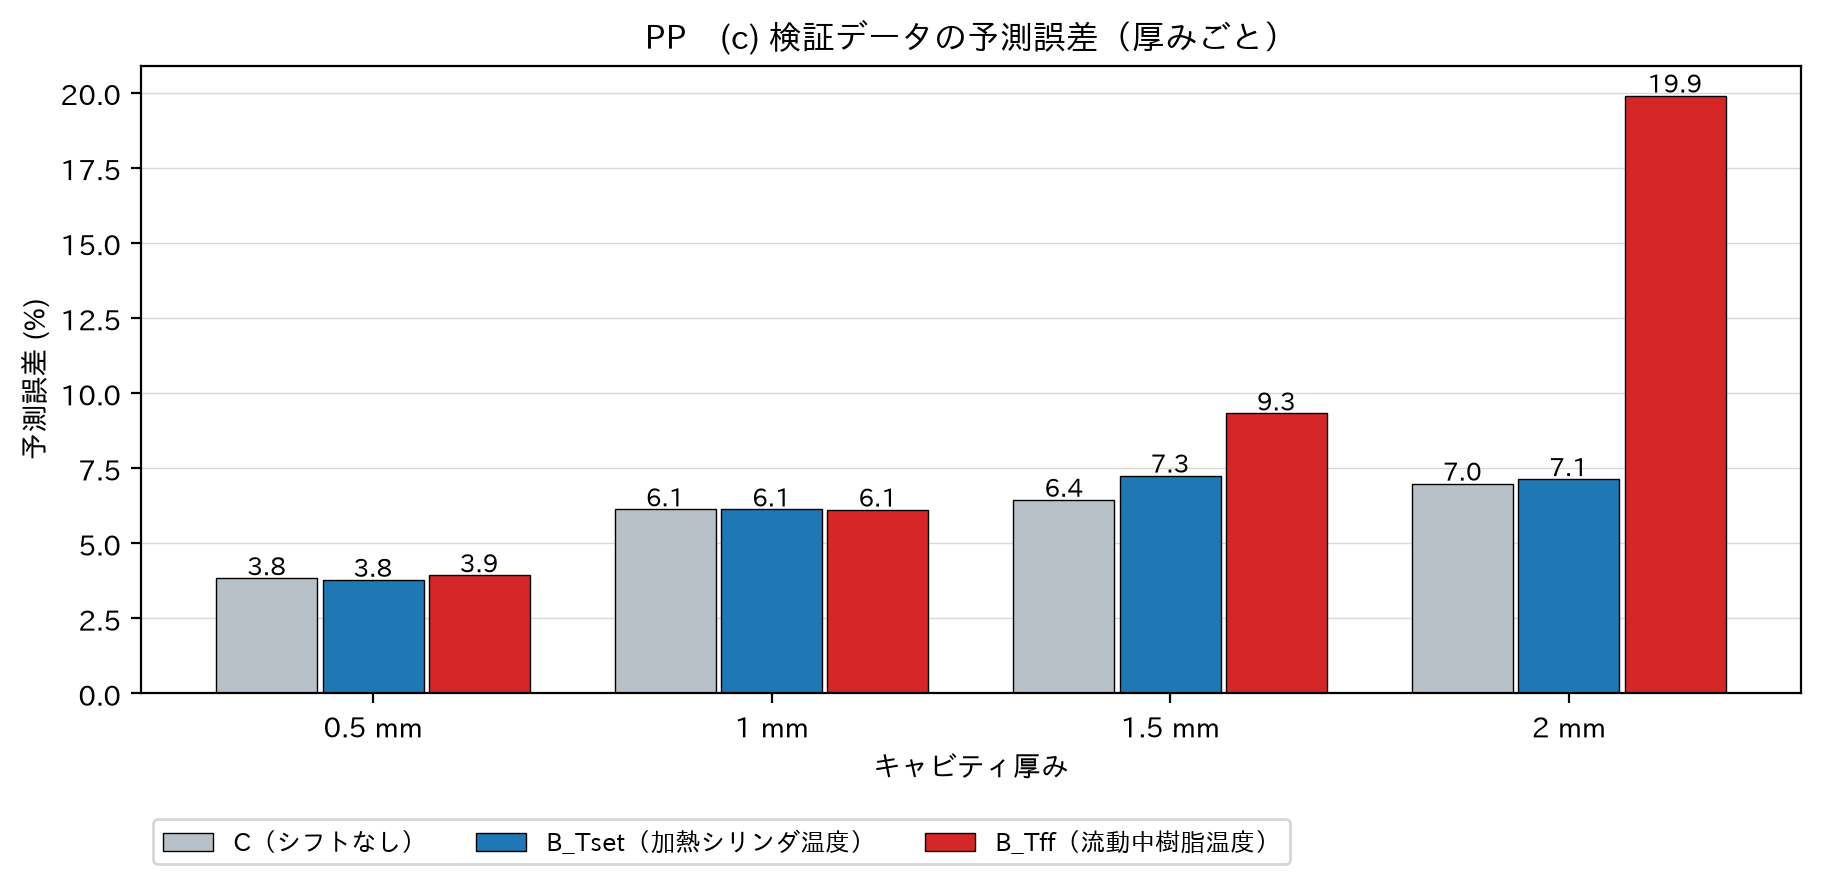
\includegraphics[width=0.95\linewidth]{01_バージンPP再々実験/01_バージンPP再々実験_学習結果/条件平均の入力/厚みごとの比較/検証誤差_厚みごと.png}
\caption{元のノート（総合データで学習）の 3 モデルの、3data の予測誤差を厚みごとに集計したもの}
\end{figure}
\begin{points}
\pt{何を示す図か}学習に用いていない 3data（射出速度の両端）の予測誤差を、厚みごとに比べる図です（基準 (c)。ファイル：\file{検証誤差_厚みごと.png}）。
\pt{軸と記号}縦軸が予測誤差（粘度の \%）。灰が C（シフトなし）、青が B\_Tset、赤が B\_Tff。
\pt{見るポイント}青と赤の差が 1.0 ポイント以上あるか。
\pt{今回の結果}薄肉（0.5・1.0 mm。3data は高速側だけ）は、3 モデルとも同じです。差が出るのは厚肉（1.5・2.0 mm。低速側の外挿を含む）で、PP は加熱シリンダ温度（B\_Tset）が小さく（2.0 mm：7.1\% 対 19.9\%）、粉砕材混合 PP と GPPS は流動中樹脂温度（B\_Tff）が小さい結果でした（粉砕材混合 PP の 2.0 mm：13.0\% 対 4.4\%）。材料によって向きが逆で、外挿の当たり外れの影響が大きい基準です。
\end{points}

\subsection{図8：厚みごとのモデルと総合データのモデル（粉砕材混合 PP・B\_Tff）}
\begin{figure}[H]
\centering
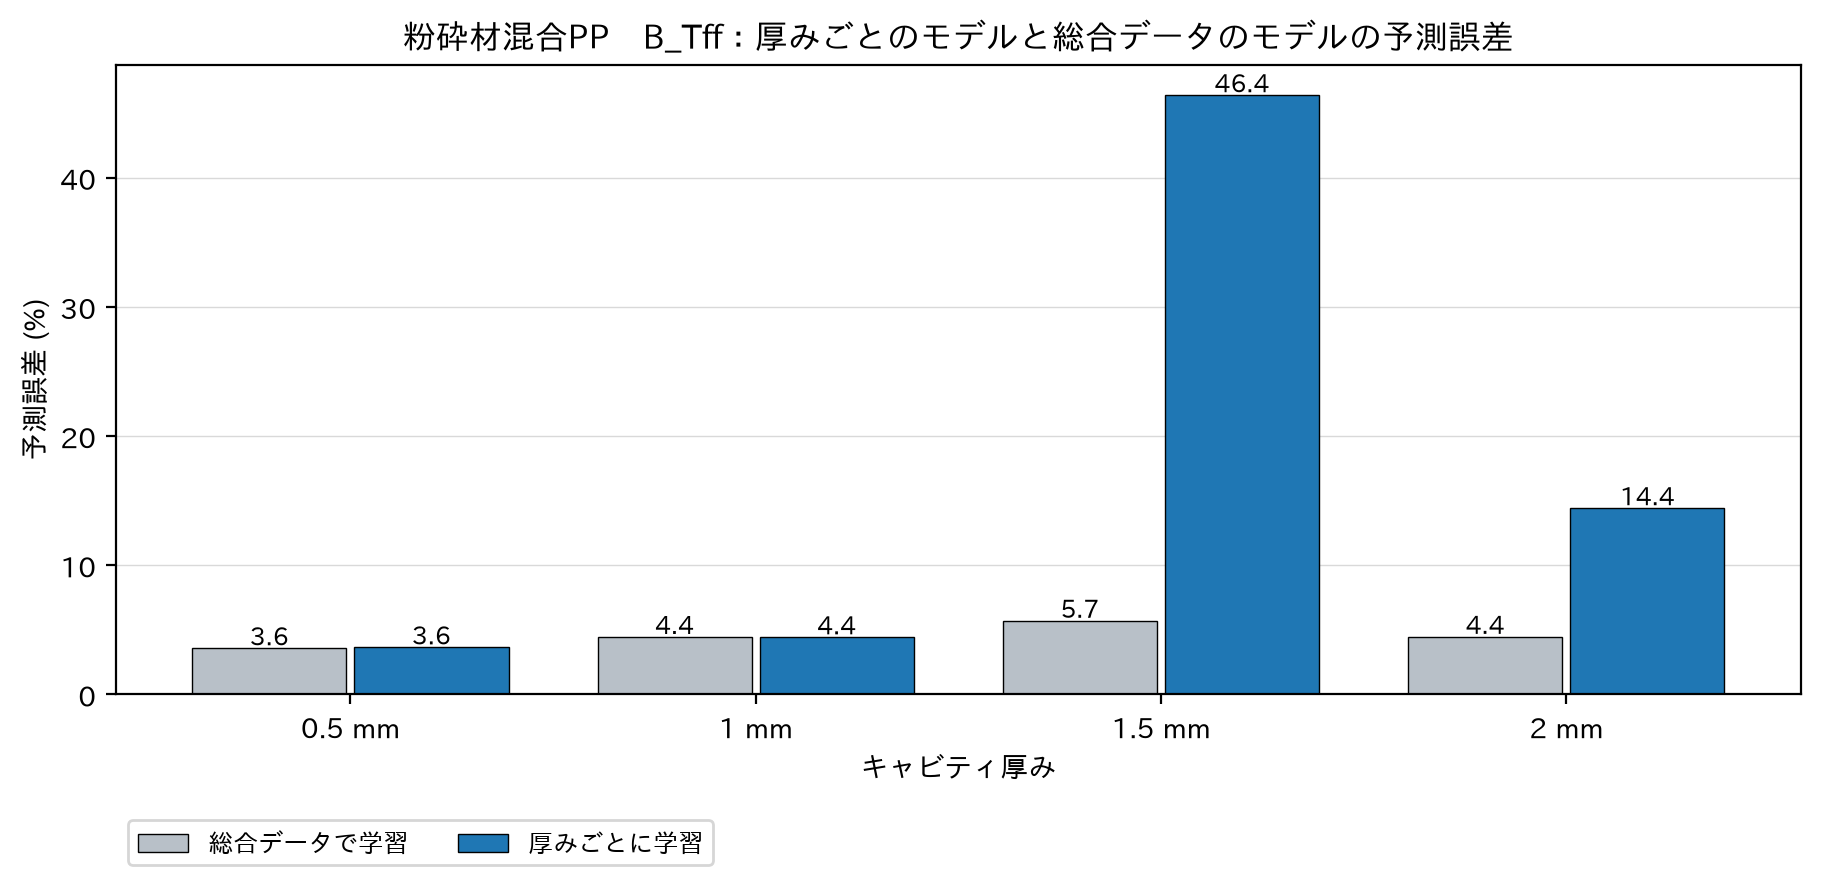
\includegraphics[width=0.9\linewidth]{02_粉砕材混合PP実験/02_粉砕材混合PP実験_学習結果/条件平均の入力/厚みごとの比較/厚みごとと総合_B_Tff.png}
\caption{灰：総合データ（全厚みの 5data）で学習、青：その厚みの 5data だけで学習。3data の予測誤差}
\end{figure}
\begin{points}
\pt{何を示す図か}学習のしかただけを変えて、同じ 3data の予測誤差を比べる図です（問い 3。ファイル：\file{厚みごとと総合_<モデル>.png}。モデルごとに 1 枚）。
\pt{軸と記号}縦軸が予測誤差（粘度の \%）。横軸がキャビティ厚み。
\pt{見るポイント}青の棒（厚みごと）が灰の棒（総合）より低いか。
\pt{今回の結果}粉砕材混合 PP の B\_Tff では、薄肉はほぼ同じですが、厚肉で厚みごとのモデルが大きく外れます（低速側の誤差：厚みごと 52\%、総合 6\%）。3 材料 $\times$ 3 モデルの 9 組のうち 8 組で、全厚みの誤差は総合データのほうが小さくなりました（5 章の表 6）。例外は PP の B\_Tff（厚みごと 10.7\%、総合 13.1\%。総合データの 2.0 mm の低速側が大きく外れるため）です。
\end{points}


% =====================================================================
\section{表の見方}


\subsection{温度シフトの確認（問い 1。全厚み共通の係数）}
\begin{table}[H]
\caption{厚みごとの温度による粘度の比 $R$ と、重ね合わせのずれ（粘度の \%）。「予測」「換算後」「判定」は、左が B\_Tset、右が B\_Tff}\label{tab:check}
\scriptsize
\begin{tabularx}{\linewidth}{@{}llrrrrrrrcc@{}}
\toprule
材料 & 厚み (mm) & 条件数 & $R$ 実測 & $R$ 予測 & $R$ 予測 & 換算前 & 換算後 & 換算後 & 判定 & 判定 \\
 & & & & B\_Tset & B\_Tff & & B\_Tset & B\_Tff & B\_Tset & B\_Tff \\
\midrule
PP & 0.5 & 26 & 1.125 & 1.118 & 1.118 & 3.9 & 7.9 & 2.1 & △ & ○ \\
 & 1.0 & 30 & 1.185 & 1.190 & 1.192 & 6.1 & 7.4 & 1.8 & △ & ○ \\
 & 1.5 & 33 & 1.220 & 1.239 & 1.238 & 7.4 & 6.3 & 2.1 & ○ & ○ \\
 & 2.0 & 36 & 1.223 & 1.236 & 1.236 & 8.7 & 6.5 & 4.7 & ○ & ○ \\
\midrule
粉砕材混合 PP & 0.5 & 27 & 1.125 & 1.110 & 1.113 & 3.9 & 9.1 & 1.5 & △ & ○ \\
 & 1.0 & 30 & 1.161 & 1.172 & 1.172 & 5.5 & 9.9 & 1.7 & △ & ○ \\
 & 1.5 & 36 & 1.228 & 1.244 & 1.230 & 8.4 & 11.7 & 4.2 & △ & ○ \\
 & 2.0 & 36 & 1.237 & 1.249 & 1.248 & 9.2 & 12.0 & 5.2 & △ & ○ \\
\midrule
GPPS & 1.0 & 30 & 1.331 & 1.331 & 1.330 & 9.9 & 7.9 & 3.1 & ○ & ○ \\
 & 1.5 & 36 & 1.404 & 1.452 & 1.444 & 13.3 & 9.7 & 5.6 & ○ & ○ \\
 & 2.0 & 36 & 1.426 & 1.441 & 1.447 & 14.4 & 9.2 & 5.5 & ○ & ○ \\

\bottomrule
\end{tabularx}
\end{table}
\begin{points}
\pt{読み方}条件数は、5data と 3data を合わせた成形条件の数。$R$ の予測が実測に近く、換算後のずれが換算前より小さければ ○ です。B\_Tff は全厚みで ○、B\_Tset は、換算でずれが増える厚みが △ です（$R$ はどちらも実測と合う）。
\end{points}

\subsection{シフトに使う温度（問い 2）}
\begin{table}[H]
\caption{厚みごとの 3 つの基準。数値は「加熱シリンダ温度／流動中樹脂温度」。(a) の係数は「横, 縦」（PP・粉砕材混合 PP は kJ/mol、GPPS は $A_1$）。右端が多数決}\label{tab:win}
\scriptsize
\begin{tabularx}{\linewidth}{@{}llrXcrcrcc@{}}
\toprule
材料 & 厚み & (a) ずれ (\%) & (a) 係数 & (a) & (b) $\Delta L$ & (b) & (c) 誤差 (\%) & (c) & 多数決 \\
\midrule
PP & 0.5 & 1.8／1.3 & 4, 12／8, 23 & $\Tff$ & +0.3 & 差なし & 3.8／3.9 & 差なし & \textbf{差なし} \\
 & 1.0 & 1.6／1.2 & 5, 15／5, 16 & 差なし & +0.1 & 差なし & 6.1／6.1 & 差なし & \textbf{差なし} \\
 & 1.5 & 1.8／2.0 & 7, 18／6, 17 & 差なし & +1.6 & 差なし & 7.3／9.3 & $\Tset$ & \textbf{差なし} \\
 & 2.0 & 4.3／4.5 & 7, 17／9, 19 & 差なし & -0.8 & 差なし & 7.1／19.9 & $\Tset$ & \textbf{差なし} \\
\midrule
粉砕材混合 PP & 0.5 & 1.7／1.1 & 4, 13／7, 21 & $\Tff$ & +0.4 & 差なし & 3.6／3.6 & 差なし & \textbf{差なし} \\
 & 1.0 & 1.8／1.5 & 4, 13／3, 12 & 差なし & +0.4 & 差なし & 4.5／4.4 & 差なし & \textbf{差なし} \\
 & 1.5 & 3.7／4.1 & 9, 21／10, 22 & 差なし & +0.3 & 差なし & 10.8／5.7 & $\Tff$ & \textbf{差なし} \\
 & 2.0 & 4.8／4.8 & 7, 17／13, 24 & 差なし & -0.2 & 差なし & 13.0／4.4 & $\Tff$ & \textbf{差なし} \\
\midrule
GPPS & 1.0 & 2.7／1.8 & 3, 8／3, 9 & $\Tff$ & +1.3 & 差なし & 7.8／7.8 & 差なし & \textbf{差なし} \\
 & 1.5 & 5.4／5.0 & 2, 7／3, 9 & 差なし & -0.8 & 差なし & 22.7／12.5 & $\Tff$ & \textbf{差なし} \\
 & 2.0 & 5.6／5.3 & 2, 7／4, 10 & 差なし & +0.2 & 差なし & 12.0／6.1 & $\Tff$ & \textbf{差なし} \\

\bottomrule
\end{tabularx}
\end{table}
\begin{points}
\pt{読み方}(a) は 5data＋3data の点で、(b) は 5data だけで、(c) は元のノート（総合データで学習）の 3data の予測で決めています。「—」は、比べられなかったもの。
\end{points}

\begin{table}[H]
\caption{(b) 厚みごとのプロファイル尤度。係数は「横, 縦」。$^{*}$ は、細かい格子の取り直しが収束しなかった（または格子の端に当たった）もの。$\Delta L$ は B\_Tff − B\_Tset}\label{tab:prof}
\scriptsize
\begin{tabularx}{\linewidth}{@{}llrXrXrr@{}}
\toprule
材料 & 厚み & 学習の条件数 & B\_Tset の係数 & 係数 0 との差 & B\_Tff の係数 & 係数 0 との差 & $\Delta L$ \\
\midrule
PP & 0.5 & 21 & 10, 25 & 2.3 & 9, 22 & 3.3 & +0.3 \\
 & 1.0 & 24 & 5, 15 & 1.4 & 5, 20 & 5.2 & +0.1 \\
 & 1.5 & 24 & 6, 16 & 2.8 & 4, 14 & 1.8 & +1.6 \\
 & 2.0 & 24 & 4, -36$^{*}$ & 3.1 & 7, 21 & 2.4 & -0.8 \\
\midrule
粉砕材混合 PP & 0.5 & 21 & 5, 15 & 2.7 & -1, -1 & 2.1 & +0.4 \\
 & 1.0 & 24 & 1, -6 & 2.3 & 3, 11 & 0.9 & +0.4 \\
 & 1.5 & 24 & 5, 13 & 3.8 & 2, 34 & 4.1 & +0.3 \\
 & 2.0 & 24 & 6, 5 & 1.8 & 7, 2 & 1.7 & -0.2 \\
\midrule
GPPS & 1.0 & 24 & 3, 6 & 1.8 & 0, 5 & 3.3 & +1.3 \\
 & 1.5 & 24 & 3, 7 & 3.5 & 2, 6 & 1.6 & -0.8 \\
 & 2.0 & 24 & 2, 3 & 2.0 & 2, 6 & 2.7 & +0.2 \\

\bottomrule
\end{tabularx}
\end{table}
\begin{points}
\pt{読み方}係数 0 との差が 3 未満なら、その厚みのデータだけでは、シフトを入れた効果がはっきりしません。全厚み共通の係数（2.1 節）と比べると、厚みごとの係数はばらつきが大きく、負の値（低温ほど粘度が低い向き）も出ます。
\end{points}

\subsection{厚みごとに学習するか、総合データで学習するか（問い 3）}
\begin{table}[H]
\caption{全厚みの 3data の予測誤差（粘度の \%）と、95\% 予測区間に入った割合。数値は「厚みごとに学習／総合データで学習」。総合が小さいものを太字}\label{tab:tt}
\scriptsize
\begin{tabularx}{\linewidth}{@{}llXXXX@{}}
\toprule
材料 & モデル & 全体 & 低速側 & 高速側 & 区間に入った割合 \\
\midrule
PP & C & 21.6／\textbf{6.3} & 41.5／\textbf{7.6} & 7.0／\textbf{5.6} & 0.87／0.90 \\
 & B\_Tset & 17.9／\textbf{6.6} & 33.2／\textbf{8.6} & 7.1／\textbf{5.5} & 0.85／0.91 \\
 & B\_Tff & 10.7／13.1 & 17.0／23.7 & 6.8／\textbf{5.6} & 0.88／0.89 \\
\midrule
粉砕材混合 PP & C & 10.5／\textbf{7.8} & 17.4／\textbf{12.6} & 4.9／\textbf{4.0} & 0.93／0.98 \\
 & B\_Tset & 15.1／\textbf{10.0} & 26.5／\textbf{17.0} & 5.0／\textbf{4.1} & 0.91／0.98 \\
 & B\_Tff & 27.3／\textbf{4.8} & 51.5／\textbf{6.1} & 5.2／\textbf{4.0} & 0.78／0.98 \\
\midrule
GPPS & C & 15.2／\textbf{11.9} & 23.6／\textbf{17.5} & 6.9／\textbf{6.6} & 0.91／0.94 \\
 & B\_Tset & 23.2／\textbf{16.3} & 38.2／\textbf{25.8} & 7.1／\textbf{6.6} & 0.90／0.86 \\
 & B\_Tff & 16.0／\textbf{9.4} & 25.0／\textbf{12.8} & 7.0／\textbf{6.6} & 0.90／0.93 \\

\bottomrule
\end{tabularx}
\end{table}
\begin{points}
\pt{読み方}厚みごとの値は、各厚みのモデルの予測を、全厚みについてまとめて計算したもの。厚みごとの内訳は \file{厚みごとと総合の比較.csv} にあります。低速側（3・5 mm/s）は厚肉（1.5・2.0 mm）だけのデータです。
\end{points}


% =====================================================================
\section{結論と、これからの選択肢}


ノートの判定は、OK 95 個、★ 7 個でした（★ は 4 温度シフトの確認・6 (b) プロファイル尤度 の節）。以下、結果をまとめます。

\begin{enumerate}[itemsep=0.8ex,topsep=0.6ex]
\item \textbf{問い 1：温度シフトは効いているか}：発表資料で使った B\_Tff（流動中樹脂温度でシフト）は、3 材料の 11 厚みすべてで ○ でした。どの厚みでも、温度の順序は実測と同じで、温度による粘度の比 $R$ も実測と合い（差は最大 0.034。ノイズの標準偏差より小さい）、全厚み共通の係数で換算すると、重ね合わせのずれが減ります（PP 3.9〜8.7\% → 1.8〜4.7\%、粉砕材混合 PP 3.9〜9.2\% → 1.5〜5.2\%、GPPS 9.9〜14.4\% → 3.1〜5.6\%）。B\_Tset は 5 厚みで ○ で、PP の 0.5・1.0 mm、粉砕材混合 PP の全厚みでは、換算でずれが増えました（△）。
\item \textbf{問い 2：シフトに使う温度}：厚みごとに係数を決め直して比べると、3 つの基準の多数決は、11 厚みすべてで「差なし」でした（33 判定の内訳：流動中樹脂温度 7・加熱シリンダ温度 2・差なし 24）。\textbf{厚みごとに見れば、どちらの温度でもほぼ同じ}です。一方、\textbf{全厚み共通の 1 組の係数で表すなら、流動中樹脂温度のほうが適しています}（問い 1 のとおり、全厚みでずれを減らす）。加熱シリンダ温度は、温度の効果が厚みで違う（$R$ が最も薄い厚みと最も厚い厚みで、PP 1.12・1.22、粉砕材混合 PP 1.12・1.24、GPPS 1.33・1.43）ことを、1 組の係数では表しきれません。流動中樹脂温度は、厚みや射出速度ごとに値が変わるので、この違いの一部を担えます。
\item \textbf{解釈の注意}：流動中樹脂温度は、せん断発熱で射出速度とともに変わります。流動中樹脂温度でのシフトは、「温度の違い」だけでなく「曲線の形の調整」（発熱の効果）も兼ねている可能性があります。(b) の対数周辺尤度で差が出なかったことも、厚みごとのデータでは、2 つの温度の役割を区別できないことを示しています。
\item \textbf{問い 3：厚みごとか、総合データか}：\textbf{今回のデータ（学習用 5data・検証用 3data）では、全厚みを含めた総合データで 1 つのモデルを学習するのがよい}と判断しました。理由は 3 つです。
\begin{enumerate}[label=(\roman*),itemsep=0.3ex,topsep=0.3ex]
\item 予測誤差：3 材料 $\times$ 3 モデルの 9 組中 8 組で、総合データのほうが小さい。各材料で最もよいモデルの誤差は、総合データ 6.3・4.8・9.4\%、厚みごと 10.7・10.5・15.2\%（PP・粉砕材混合 PP・GPPS）。
\item データの量：厚みごとの学習データは成形条件 21〜24 で、総合データ（72〜93）の約 1/4。シフトの係数がよく決まらず（係数 0 との差 0.9〜5.2）、厚みで大きく変わります。
\item 外挿：差が大きいのは厚肉の低速側（学習範囲の外）で、総合データは、ほかの厚みの傾向も使えます。薄肉（3data は高速側だけ）の差は最大 0.4 ポイントで、ほとんどありません。また、厚みごとのモデルは、学習していない厚みを予測できません。
\end{enumerate}
例外は PP の B\_Tff で、厚みごとのほうが小さい（10.7\% 対 13.1\%）結果でした。ただし、PP では、総合データで学習した C（6.3\%）のほうがさらに小さくなります。
\item \textbf{ノートの ★ の意味}：(4 節) B\_Tset で、全厚み共通の係数で換算すると、ずれが増える厚みがある（問い 1 の △）。(6 節) 厚みごとのプロファイル尤度で、最良の点が動き続け、細かい格子の取り直しが収束しなかった（尤度の面が平らで、係数が決まりにくい）。エラーではなく、結果を読むときの注意点です。
\end{enumerate}

\subsection{これからの選択肢（ユーザーの判断）}
\begin{enumerate}[itemsep=0.6ex,topsep=0.6ex]
\item \textbf{PP の主のモデル}：PP では、総合データで学習した B\_Tff の 3data の誤差（13.1\%）が、C（6.3\%）・B\_Tset（6.6\%）より大きく、主に 2.0 mm の低速側の外挿で外れます。発表資料は 3 材料とも B\_Tff で示しました。PP だけ別のモデルを示すかは、ご判断ください（元のノートの説明書のとおり、外挿の優劣は最適化の局所解にも左右されます）。
\item \textbf{厚みごとに学習したい場合}：1 つの厚みで係数を決めるには、成形条件（射出速度・温度の水準）を増やす必要があります。ショット数を増やしても、成形条件の数は増えないので、係数の決まりやすさはほとんど変わりません。
\end{enumerate}


\end{document}
